\documentclass[a4paper,12pt]{article}
\usepackage[a4paper, total={180mm, 272mm}]{geometry}

\usepackage{fontspec}
\setmainfont[Path=fonts/, Extension=.ttf]{ipaexm}

\setlength\parindent{3.5em}
\setlength\parskip{0em}
\renewcommand{\baselinestretch}{1.247}

\usepackage{eepic}

\usepackage{tikz}

\begin{document}

\thispagestyle{empty}

\Large
\noindent \\
Level Auto Ino\medskip
\par
\normalsize
Spread the maximum brightness range of the picture.\\
\par
Also does automatic level correction such as to brighten the image for a dark mask.\\
\par
Based on the brightest value and the darkest value of the input image,\par
it spreads the brightness range of the darkest value (Out Min) and the\par
brightest value (Out Max) as a numerical value.\par
-{-}> \textquotedbl Level Auto Figure 1 Calculation View\textquotedbl \ reference\\
\par
Since it expands the range of each RGBA channel, it does not take into account\par
the RGBA\textquotesingle s balance. Therefore please note that it may change colors, in a colored\par
image.\\
\par
When you check the results, please do not use the sub-camera.\par
Since the sub-camera in the range of the input image is different, it changes the\par
darkest and brightest values of the input image, it can not be accurately processed.\\
\\
-{-}- \ Inputs \ -{-}-\\
Source\par
Connect the image to process.\\
\\
-{-}- \ Settings \ -{-}-\\
In Min Shift\\
In Max Shift\par
Minimum and maximum values of the input image Pixel is automatically calculated,\par
 and adjusted by adding to its value.\par
For example, if there is only one placed bright Pixel, when you want to ignore it,\par
spread the range by specifying a negative \textquotedbl In Max Shift\textquotedbl \ value.\par
Pixel value (8 or 16bits) is specified as a value of 0 to 1.\par
Minimum value is -1, maximum value is 1.\par
\noindent \hskip 7em Min \ \ \ \ \, 0\par
\noindent \hskip 7em Max \ \ \ \ -1\par
These values will make the screen become black.\par
\noindent \hskip 7em Min \ \ \ \ \, 1\par
\noindent \hskip 7em Max \ \ \ \ \ 0\par
If you use these values, the screen will become pure white.\par
If you use a value of 0 for both, there will be no adjustment by the shift.\par
The default values for both are 0.\\
\\
Out Min

\newpage

\thispagestyle{empty}

\ \vspace{-0.2em}
\par
\noindent Out Max\par
Determines the darkest value of the output image (minimum value) and the\par
brightest value (maximum value).\par
Minimum value is 0, maximum value is 1.\par
The defaults are\par
\noindent \hskip 7em Out Min is 0\par
\noindent \hskip 7em Out Max is 1\par
for the values.\\
\\
Gamma\par
Used for the gamma correction between \textquotedbl Out Min\textquotedbl \ and \textquotedbl Out Max\textquotedbl .\par
A Value between 0.1 and 1.0, will make the image become darker.\par
It does not compensate when you specify a value of 1.0.\par
A value between 1.0 and 10.0, will make the image become brighter.\par
The default value is 1.\\
\\
Level Auto Figure 1 \ \ Calculation View

\large
\noindent \begin{picture}(0,0)
\linethickness{0.01em}
\put(18.5,-94){\line(0,-1){81}}
\put(18.5,-94){\line(-2,-3){4}}
\put(18.5,-94){\line(2,-3){4}}
\put(18.5,-175){\line(-2,3){4}}
\put(18.5,-175){\line(2,3){4}}

\put(114,-22){\line(0,-1){199}}
\put(256,-22){\line(0,-1){199}}
\put(85,-51){\line(1,0){199}}
\put(85,-193){\line(1,0){199}}

\put(101,-7){\small{IN}}
\put(233,-7){\small{OUT}}
\put(290,-51){\small{1}}
\put(290,-193){\small{0}}
\put(72,-91){\small{max}}
\put(258,-69){\small{max}}
\put(116,-105){\small{max\_shift}}
\put(116,-176){\small{min\_shift}}
\put(72,-188){\small{min}}
\put(258,-188){\small{min}}
\end{picture}\\[3em]

\noindent \hskip 3.8em 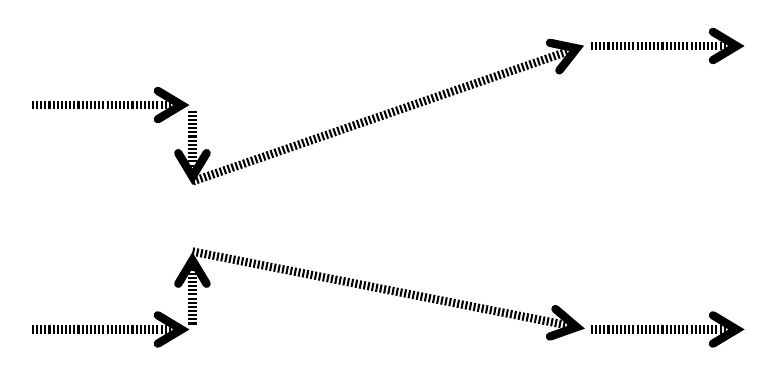
\begin{tikzpicture}[line width=3pt]
\draw[line cap=round] (1.6,-0.75) -- (1.9,-0.93) -- (1.6,-1.11);
\draw[dashed,dash pattern=on 0.75pt off 0.75pt] (0,-0.93) -- (1.9,-0.93);

\draw[line cap=round] (8.65,0) -- (8.95,-0.18) -- (8.65,-0.36);
\draw[dashed,dash pattern=on 0.75pt off 0.75pt] (7.1,-0.18) -- (8.95,-0.18);

\draw[line cap=round] (1.6,-3.6) -- (1.9,-3.78) -- (1.6,-3.96);
\draw[dashed,dash pattern=on 0.75pt off 0.75pt] (0,-3.78) -- (1.9,-3.78);

\draw[line cap=round] (8.65,-3.6) -- (8.95,-3.78) -- (8.65,-3.96);
\draw[dashed,dash pattern=on 0.75pt off 0.75pt] (7.1,-3.78) -- (8.85,-3.78);

\draw[line cap=round] (1.86,-1.54) -- (2.04,-1.84) -- (2.22,-1.54);
\draw[dashed,dash pattern=on 0.75pt off 0.75pt] (2.04,-1) -- (2.04,-1.84);

\draw[line cap=round] (1.86,-3.2) -- (2.04,-2.9) -- (2.22,-3.2);
\draw[dashed,dash pattern=on 0.75pt off 0.75pt] (2.04,-2.9) -- (2.04,-3.74);

\draw[line cap=round] (6.58,-0.14) -- (6.92,-0.21) -- (6.7,-0.49);
\draw[dashed,dash pattern=on 0.75pt off 0.75pt] (2.04,-1.9) -- (6.92,-0.21);

\draw[line cap=round] (6.65,-3.52) -- (6.92,-3.75) -- (6.58,-3.87);
\draw[dashed,dash pattern=on 0.75pt off 0.75pt] (2.04,-2.79) -- (6.92,-3.75);

\end{tikzpicture}

\end{document}